
\section{Parameters}

In 3DNA there are 3 sets of ``symmetric'' local parameters being defined
which are:

\begin{enumerate}
\item Base-pair parameters.
\item Base (Base pair) step parameters.
\item Base (Base pair) helical parameters.
\end{enumerate}

Bases or base-pairs are treated as ``rigid bodies'' using classical mechanics.

%%The first two are based on cartesian coordinates (``object centered'', reference frame),
%%whereas the third is referred as helical coordinates (non-object centered)
The first two sets of parameters are based on cartesian coordinates,
whereas the third is referred as helical coordinates, which resembles 
cylindrical coordinates and it's based on Chasles Theorem\cite{babcock1994}.

\subsection{Base-pair and Base-step Parameters Calculation}
In 3DNA  \footnote{Note: Olson2001\cite{olson2001} Gives  the standard
reference   frame  definition   on  which   the  calculation   of  the
parameters\cite{lu2003}, \cite{lu1997}  is based.}  you  start using a
pdb file  which is  completely experimental\footnote{This is  the most
common case  but the pdb  file can also  be the result  of theoretical
modeling}, you download  this from the ndb or  pdb, this file contains
the experimentally obtained cartesian  coordinates of the atoms.  With
this  experimental data  you  do a  least  squares fit  to a  standard
reference           frame           as          described           at
http://rutchem.rutgers.edu/\~{}olson/jmb/ls\_fit.html  or at  the 3DNA
manual technical details  section or at Olson2001\cite{olson2001}, you
can       also       use        the       octave       script       at
http://rutchem.rutgers.edu/\~{}esguerra/RNA/scripts.html as a tutorial
example. 
It seems that the  coordinate origin which is embedded in the
standard reference frame definition is kept, and is used for both base
and base-pairs.  In the case of  single bases, not  base-pairs, it seems
that you just keep the  origin of coordinates of an ideal Watson-Crick
pair, the definition  of this frame can be seen  in Figure II.  Before
Olson2001\cite{olson2001} there were various options for the selection
of the coordinates origin, one example is that of lu1997\cite{lu1997},
where  the  reference  frames  for  base-pairs and  single  bases  are
different and were defined as  given by Figure I.  This definition was
modified  to  a  standard  reference  frame which  is  good  for  both
base-pairs and single bases and is illustrated in Figure II.

\begin{figure}[htbp]
\centering
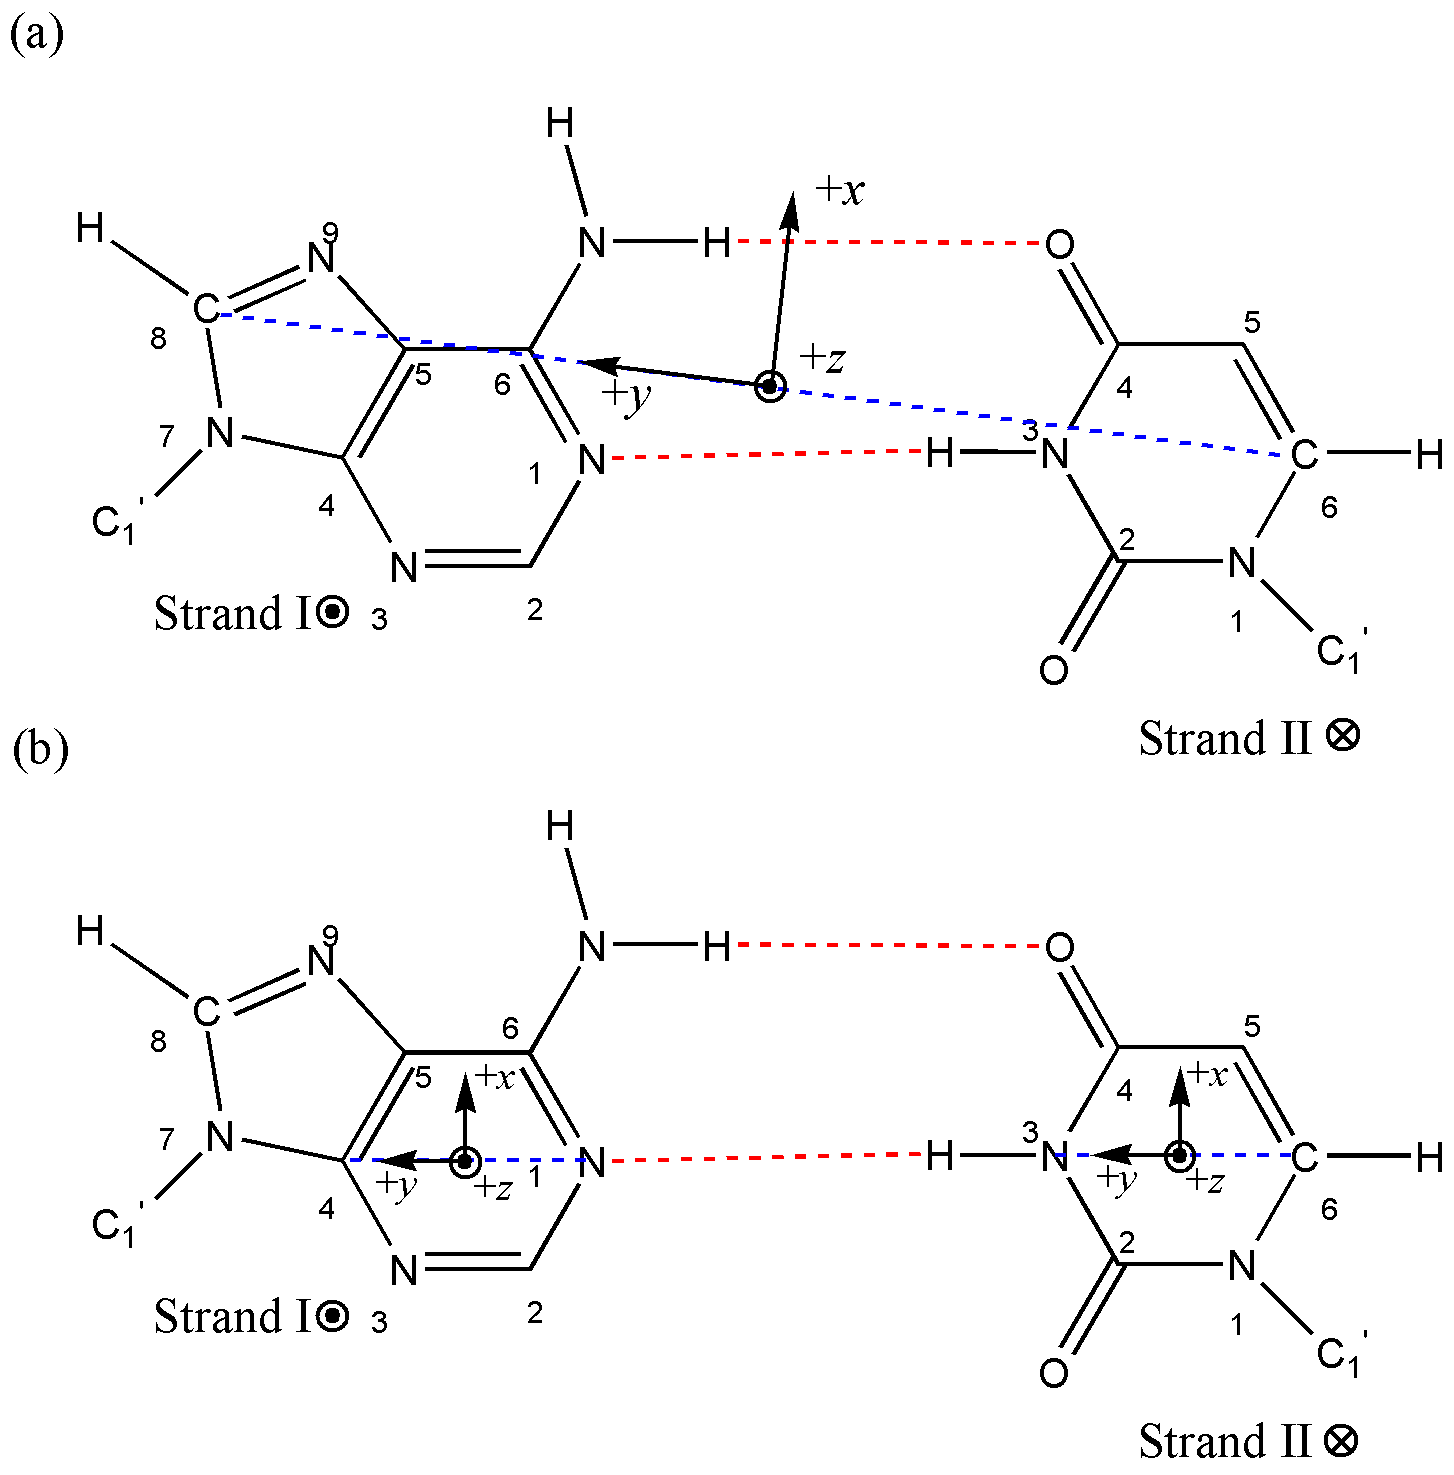
\includegraphics[scale=0.8]{baseandbasepair.png}
\caption{SCHNAaP Reference Frame}
\end{figure}

\begin{figure}[htbp]
\centering
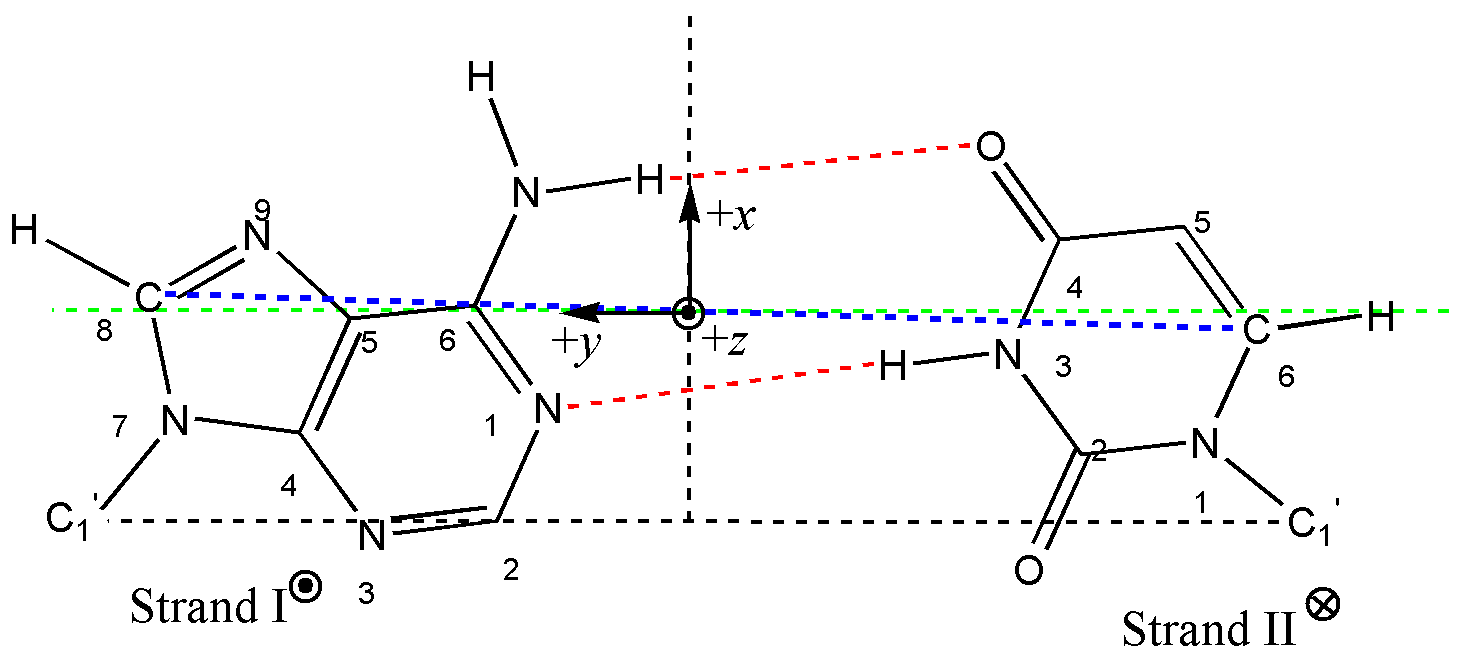
\includegraphics[scale=0.8]{standard.png}
\caption{Standard Reference Frame}
\end{figure}

Once you have  figured out the coordinate origins  for two consecutive
bases or  base-pairs comprising a step you  proceed to define a middle
 step  triad (MST) \cite{lu1997}.

This can be described by the following procedure:

1) Find  the angle between  consecutive z-axis.  Since these  are unit
vectors, then from dot product definition:

\begin{gather}
\Gamma = \cos^{-1} (\hat{z}_i \cdot \hat{z}_{i+1})
\end{gather}


2) Then find the vector which  results from doing the cross product of
consecutive z-axis (that  is, the normal to the plane  formed by the 2
vectors), this is called the Roll-Tilt axis and then normalize to make
it a unit vector $\hat{rt}$,

\begin{gather}
rt = \hat{z}_i \times \hat{z}_{i+1}
\end{gather}

%% Note: Why do you need a matrix? Isn't this always in 3D and therefore 
%% just vectors would do? Why the more general matricial way instead of
%% the vectorial representation?
3) To  make the  two  consecutive z  vectors  coincide, you use can just
use a linear homogeneous transformation of the plane so that the  original
orientation matrices $T_i$ and $T_{i+1}$ are rotated $ \pm \Gamma / 2$
degrees  by  $R_{rt}(\theta)$ to  get  the  transformed $T_i^{'}$  and
$T_{i+1}^{'}$ orientation matrices.
%% NEED to include GRAPHICS of ANGLES and COORDINATES in general.

\begin{gather}
T_i^{'} = R_{rt}(\theta) T_{i} \\ T_{i+1}^{'} = R_{rt}(\theta) T_{i+1}
\end{gather}

The  origin of  coordinates for  the MST  is just  the average  of the
position vectors for the $i$ and $i+1$ reference frames,

\begin{gather}
r_{mst} = \frac{(r_i + r_{i+1})} {2}
\end{gather}

4) Again  using the dot  product you  can find  the angle  between the
transformed $\hat{y}^{'}$ vectors and this is just the Twist ($\Omega$) and
also if you just do the dot product of the $\hat{z}_{mst}$ unit vector with 
the vector resulting of the cross product of $\hat{y}_{i}^{'}$ and $\hat{y}_{i+1}^{'}$ you 
get the sign of $\Omega$. Since the transformed x-y plane is orthogonal to $\hat{z}$ then
this applies in the same manner for x,
%%The vector resulting from (yi X yi+1 has got to be parallel or anti-parallel to zMST,
%%there's no other possibility.

\begin{gather}
\Omega = cos^{-1}(\hat{y}_{i}^{'} \cdot \hat{y}_{i+1}^{'})\\
(\hat{y}_{i}^{'} \times \hat{y}_{i+1}^{'}) \cdot \hat{z}_{mst} > 0, \quad then \ \Omega > 0\\
(\hat{y}_{i}^{'} \times \hat{y}_{i+1}^{'}) \cdot \hat{z}_{mst} < 0, \quad then \ \Omega < 0
\end{gather}

if normalized beforehand then the rule should be,

\begin{gather}
(\hat{y}_{i}^{'} \times \hat{y}_{i+1}^{'}) \cdot \hat{z}_{mst} = 1, \quad then \ \Omega > 1\\
(\hat{y}_{i}^{'} \times \hat{y}_{i+1}^{'}) \cdot \hat{z}_{mst} = -1,\quad then \ \Omega < -1
\end{gather}

5) With more dot product we can find other angles, like one called $\phi$,
%% Show in figure.

\begin{gather}
\phi = cos^{-1}(\hat{rt} \cdot \hat{y}_{mst})\\
(\hat{rt} \times \hat{y}_{mst}) \cdot \hat{z}_{mst} > 0, \quad then \ 180 \geq \phi \geq 0\\
(\hat{rt} \times \hat{y}_{mst}) \cdot \hat{z}_{mst} < 0, \quad then \ -180 \leq \phi \leq 0
\end{gather}

and then, 
%as if we were doing a change of variables from cartesian to polar.

\begin{gather}
\rho = \Gamma cos (\phi)\\
\tau = \Gamma sin (\phi)
\end{gather}

which are the remaining angular degrees of freedom for step parameters.

Now to get the remaining 3 translational degrees of freedom for step parameters one just
needs to do:

\begin{gather}
[D_xD_yD_z]=(r_{i+1} - r_{i})T_{mst}
\end{gather}

To get the base-pair parameters the procedure is completely analogous so that
$\Omega$, $\rho$ and $\tau$ are the analogs of $\omega$, $\kappa$ and $\sigma$
now the MST is called MBT (Middle Base Triad) and the axis which are made to 
coincide are the y-axis and not the z-axis as in the base-step case,

\begin{gather}
\gamma = \cos^{-1} (\hat{y}_{iII} \cdot \hat{y}_{iI})\\
bo = \hat{y}_{iII} \times \hat{y}_{iI}\\
\hat{bo} = \frac {bo}{\sqrt{bo \cdot bo}}\\
T_{iII}^{'} = R_{bo}(+\frac{\gamma}{2}) T_{iII} \\ 
T_{iI}^{'} = R_{bo}(-\frac{\gamma}{2}) T_{iI}\\
r_{mbt} = \frac{(r_{iII} + r_{iI})} {2}\\
\omega = cos^{-1}(\hat{x}_{iII}^{'} \cdot \hat{x}_{iI}^{'})\\
(\hat{x}_{iII}^{'} \times \hat{x}_{iI}^{'}) \cdot \hat{y}_{mbt} > 0, \quad then \ \omega > 0\\
(\hat{x}_{iII}^{'} \times \hat{x}_{iI}^{'}) \cdot \hat{y}_{mbt} < 0, \quad then \ \omega < 0\\
\phi^{'} = cos^{-1}(\hat{bo} \cdot \hat{x}_{mbt})\\
(\hat{bo} \times \hat{x}_{mbt}) \cdot \hat{y}_{mbt} > 0, \quad then \ 180 \geq \phi^{'} \geq 0\\
(\hat{bo} \times \hat{x}_{mbt}) \cdot \hat{y}_{mbt} < 0, \quad then \ -180 \leq \phi^{'} \leq 0\\
\kappa = \gamma cos (\phi^{'})\\
\sigma = \gamma sin (\phi^{'})\\
[S_xS_yS_z]=(r_{iI} - r_{iII})T_{mbt}
\end{gather}


\subsection{Local Helical Parameters Calculation}

In the case  of local helical parameters Chasles  theorem which states
that:
\begin{quote}
``One  can always transport a  free rigid body  from one position
and  orientation  to another  position  and  orientation  by a  single
continuous   motion   along   a    unique   axis   of   rotation''
\end{quote}
is applied\cite{babcock1994}.\footnote{So, finally, what  is actually  the local
description of the helix according to Bansal?  I haven't seen Bansal's
paper but in Babcock the definition of the helical axis vector and the
position  of the  helical axis  is  described in  all its  geometrical
detail and I wonder if this is just the same.}

3DNA calculates the helical axis  vector ($\vec{H}$) for a base or base-pair
step and  its position ($\vec{P}$).   We have made  a simple script  to draw
this along  with the RNA  backbone in KiNG  as a kinemage,  see Figure
3. or     you    can    also     download    this     kinemage    from
http://eden.rutgers.edu/\~{}esguerra/RNA/onlyrna.kin

\begin{figure}[htbp]
\centering
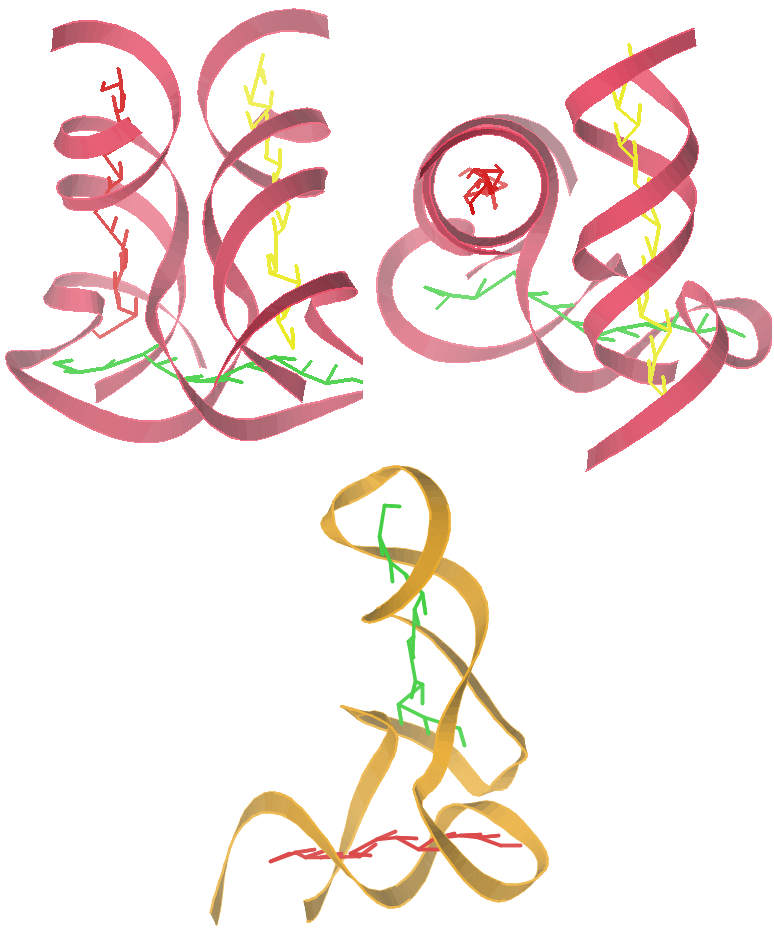
\includegraphics[scale=0.4]{both}
\caption{Helical axis vectors over RNA backbone}
\end{figure}

%% Reminder: Do for 1qu3(a tRNA) too.
One can see in Figure  3 the RNA structures 1egk(top) and 1qu3(bottom)
showing the  local helical axis  vectors in the helical  regions which
are pointing in the same direction for a particular helical region and
in relation to the ones in the following region are perpendicular like
the whole region is, therefore this  kind of maps can give you an idea
of local  bending in a graphical  way. Another way  of doing basically
the same thing but in a slightly more numerical instead of graphical way
is doing  the dot product of the helical axis vectors
between consecutive base-pairs, so  if they
are parallel or are very close to being parallel the result will be 1,
-1 for antiparallel and 0 for perpendicular as can be seen in Figure 4
also for the 1egk and 1qu3 entries of the pdb which correspond respectively 
to a four-way junction and tRNA(ILE).

\begin{figure}[htbp]
\centering
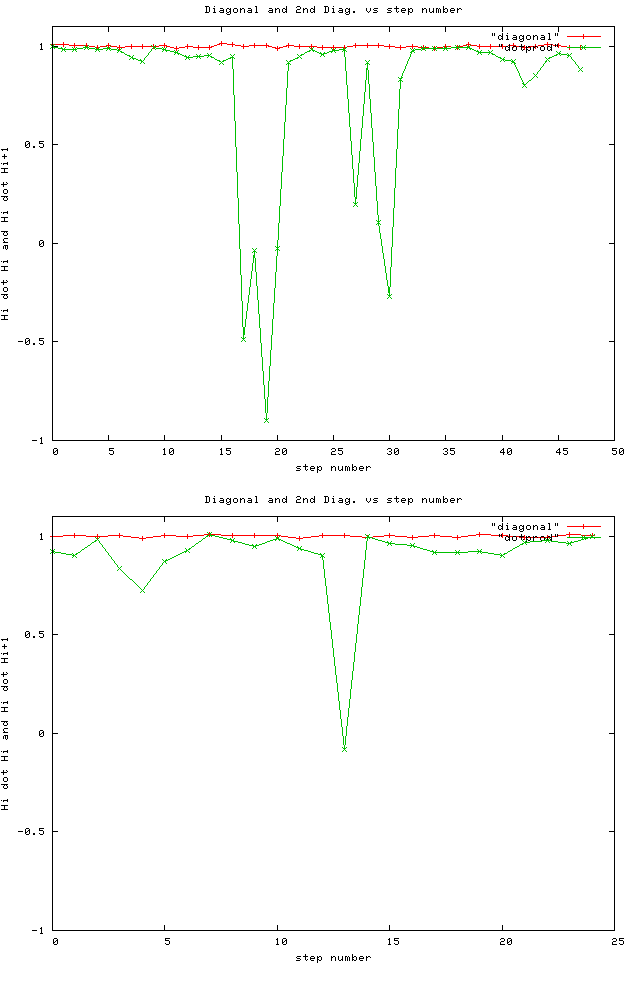
\includegraphics[scale=0.4]{normalized.png}
\caption{$H_i$ dot $H_{i+1}$ for 1egk and 1qu3} 
\end{figure}

\subsection{Global Helical Parameter Calculation}

3DNA automatically recognizes the helical regions, for example for the
50S  rRNA of \textit{haloarcula marismortui}   it recognizes  111 helical
regions and 38 of those regions are assigned as  regular helix type, that
is,  A-form, for  example, if  so, 3DNA  outputs a  file with  the axis
coordinates in raster3D format called poc\_haxis.r3d.
These regions can be rendered as cylinders as is shown in Figure V.

\begin{figure}[hb]
\centering
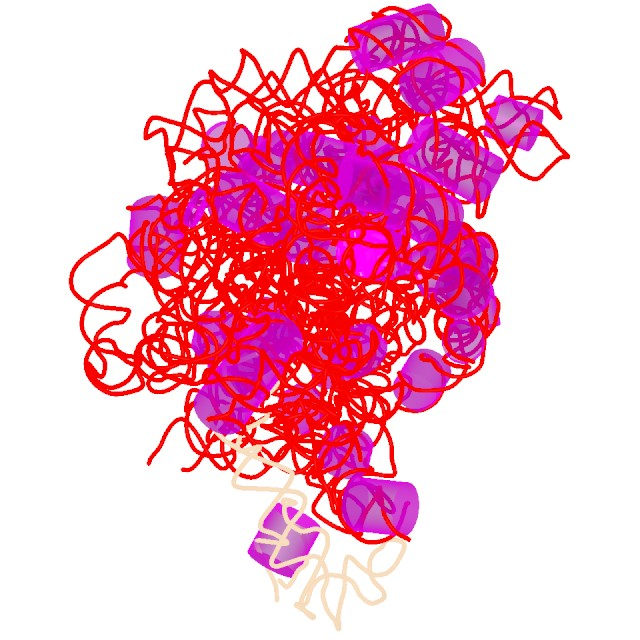
\includegraphics[scale=0.45]{cylinder.png}
\caption{Regular Helical Regions of RR0033.pdb}
\end{figure}

Other types of cylinder representation can be done for smaller regions
based on  the local helical region  vectors where we might  be able to
obtain  a   similar  representation  to  that  used   to  analyze  the
ribonuclease P ribozyme\cite{harris1997}  and also for the non-regular
helix type regions but since  there is no poc\_haxis.r3d file existent
in this cases I will have to generate a script to do this.

Ideally  one  would like  to  have an  automatic  script  to do  these
cylinder  representations  and also  a  utility  which  will draw  the
regular helix types as cylinders  only, all the helix regions, or only
the non-regular ones, etc.  One can attempt to do this with the render
utility of raster3D or perhaps it  might be better and easier to do it
using kinemage  but the generation of  cylinders seems not  to be very
clear using kinemage.

Then  one would  like to  start quantifying  the  interactions between
helical  regions  further  from  visual inspection  or  just  distance
criteria as  those exposed by Westhof  and Fritsch \cite{westhof2000}
to get and idea of tertiary interactions as a direct output of 3DNA.

